\section{User Interface Design} \label{sec:user-interface}
In this section is rapresented the UX Diagram for the User application with the purpose of showing a schema quite detailed about it. Because in our project from each page the user can go to all the other pages, to make this diagram more readable we have insert a "General Page" that incorporates all the functionalities to go to any page. For the mockups refer to the RASD.
%Provide an overview on how the user interface(s) of your system will look like; if you have included this part in the RASD, you can simply refer to what you have already done, possibly, providing here some extensions if applicable.
\begin{figure}[htbp]
\centering
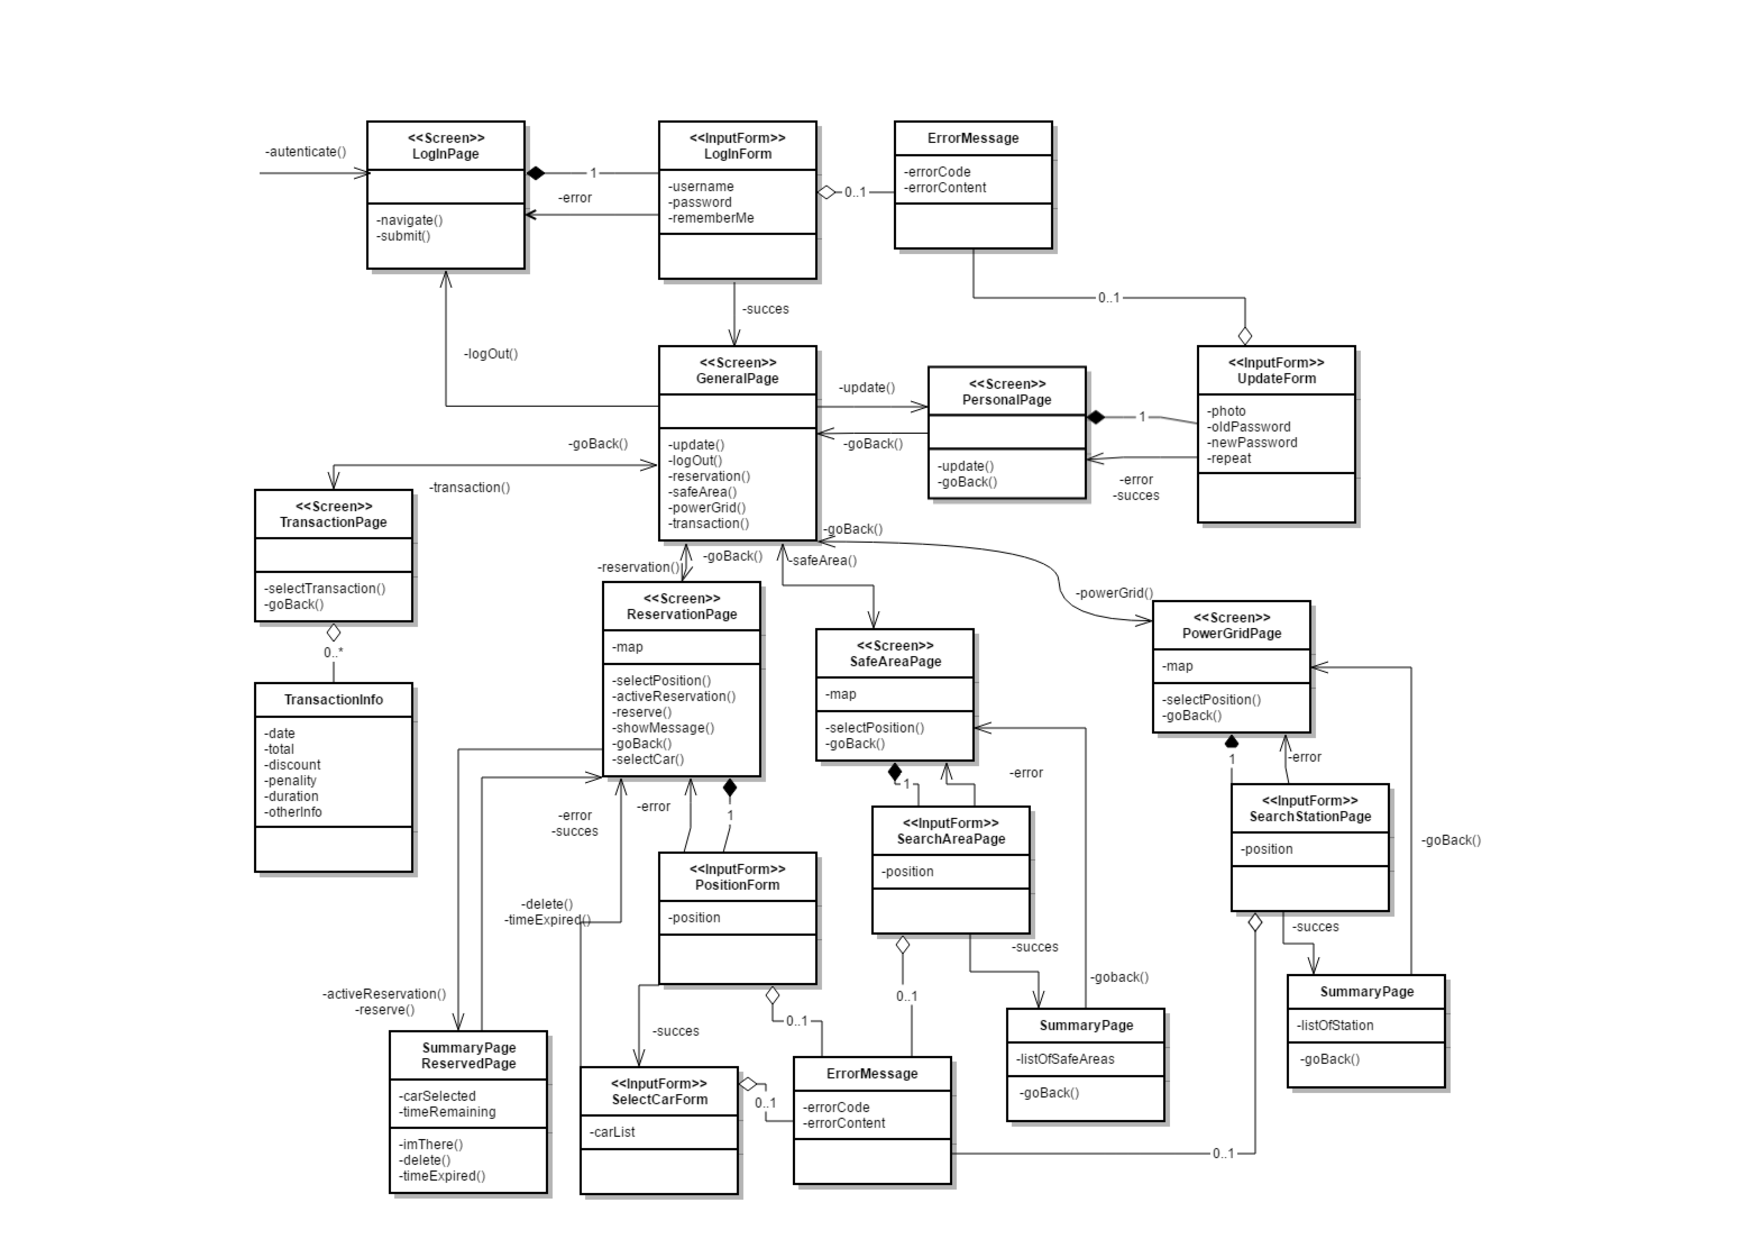
\includegraphics[width=\textwidth]{Images/UxDiagram.pdf}
\vspace{10pt}
\caption{Diagram of the user interface}
\label{fig:user-interface}
\end{figure}
\clearpage
